\chapter{Technical Background And State of Art}{
	% Article & books
	% Intro of   Fault-Tolerant Design 
	% Case study in chapter 8 of : (book) Fault tolerant Systems
	
	\section*{Safety critical application system}{
		% Article & books
		% 1.1, 1.2, 1.3 of: (book) Fault-Tolerant Design
		% Case study in chapter 8 of : (book) Fault tolerant Systems
		
		\subsection{Dependability Model}{
			% Article & books
			% chapter 2 of:  (book) Fault-Tolerant Design
			Dependability is the ability of a system to provide a predetermined level of service to the user \cite{Dubrova2013}. This capacity depends on the system application, for example a wrong use or high workload make the level of service offered go down. From the designer's point of view, the dependability of a system must be verified through tests and simulations , in order to verify the correct functioning of the system in various environment. For system that works in critical applications, in addition to the functional tests must be made tests that verify the level of service required despite environment conditions. For example in satellites it is not possible to do maintenance and the correct behavior of on-board systems is necessary to avoid the fall of the asset, so when the Dependability required to the system is high, many stress tests must be done to have a complete technical testing. For these reasons to guarantee the dependability in a given application the main factors are how the system is designed and which kind of tests is performed on it.
			
			Dependability in characterized by: Metrics, Attributes, Impairments and Means. These four categories allow us to completely define the dependability in a system and they are explained below:
			\paragraph{Dependability Metrics}{
				Dependability metrics are used to measure the dependability of a system and they are used to verify Dependability Attributes. The Metrics are experimentally measured or estimated through various techniques. These are the main metrics used: 
				\begin{itemize}
					\item \textbf{\textit{TTF} : } Time To Failure is the time to a error in a specific system \cite{Mukherjee2008}. For example a device with TTF equal to 1 year will have an error after one year of correct work.
		
					\item \textbf{\textit{MTTF} : } Mean Time To Failure is the mean time between two failure in a system. Under certain condition (e.g. formula \ref{Reliability2}) we can combine the MTTF of various parts to find the MTTF of overall system, to do this we should use the following formula:
					\begin{equation}
						MTTF_{system} = \dfrac{1}{MTTF_{part1}^{-1} + MTTF_{part2}^{-1}} = \dfrac{1}{\sum\limits_{i=0}^{n_{parts}}\frac{1}{MTTF_i}}
					\end{equation} 		
					
					\item \textbf{\textit{FIT} : } Failure In Time is the number of errors in a billion of hours. The relation between MTTF (expressed in year) and FIT is:
					\begin{equation}
					FIT = \dfrac{140000}{MTTF_{year}}
					\end{equation} 
					The FIT metric is used instead of MTTF because it makes calculation easier, in fact system FIT can be easly calculated in this way:
					\begin{equation}
					FIT_{system} = \sum_{i=0}^{n_{parts}}\,FIT_i
					\end{equation}
					
					\item \textbf{\textit{MTTR} : } The Mean Time To Recover is the time needed to a system to repair an error once it is detected  \cite{Mukherjee2008}.
					
					\item \textbf{\textit{MTBF} : } The Mean Time Between Failure is the mean time between the start/restart and an error detection, for this reason we have:
					\begin{equation}
						MTBF\;=\;MTTF+MTTR
					\end{equation}
				\end{itemize} 
			} % end Dependability Metrics
			\paragraph{Dependability Attributes}{
				Attributes are the properties which are expected from a system that experiencing faults to be dependable \cite{Dubrova2013}. These attributes are evaluated from Dependability Metrics according to a fault model. The most used Attributes are Reliability, Safety and Availability defined below: 
				\begin{itemize}
					
					\item \textbf{\textit{Reliability} : } it is the probability that a system will operate without failures in a given time interval. This type of Attribute is widely used for example in space applications, where it is necessary to guarantee operation for certain period.  At the integrated circuit level many techniques have been adopted over time to increase reliability by improving production processes, usually are used old processes experiences to predict the reliability of a new product, this is done on all ICs but especially on memories \cite{An_Extended_Building-In_Reliability_Methodology_on_Evaluating_SRAM}. Reliability can be expressed according to \textit{exponential failure law} :
					\begin{equation} \label{Reliability1}
						R(t)= e^{-h(t) \:\: t} \simeq e^{-\lambda \:\: t} 
					\end{equation} 
					Where $h(t)$ is the \textit{Instantaneous Error Rate} considered as the probability that the system has an error in a certain interval $\Delta t$ which start at instant $t$, so it is the probability of error in the time interval $(t,\, t\;+\;\Delta t )$. To simplify calculation $h(t)$ is usually approximated with the constant error rate $\lambda$, that is equal to $1/MTTF = FIT$ \cite{Mukherjee2008}.
					For these consideration when we have the FIT of each part of a system we can use formula \ref{Reliability1} to find total reliability, in this  case we consider to have $n$ independent parts each with a certain failure rate $h_i$:
					\begin{equation} \label{Reliability2}
						R(t)_{system} = \prod_{i=0}^{n-1}R_i(t) = e^{-\left(\sum_{i=0}^{n-1}h_i\right)}
					\end{equation}
					This model is valid if we consider the failure rate constant. From formula \ref{Reliability2}  we can states that the FIT of a system is equal to the sum of the FIT of each part.
					
					\item \textbf{\textit{Availability} : } It is the percentage of time the system remains active and it can be used. This Attribute is employed a lot in the IT field, for example to characterize servers or a communication network  \cite{Availability_requirement_for_a_fault-management_server_in_high-availability_communication_system} \cite{Guaranteeing_High_Availability_to_Client-Server_Communications}. It is therefore required in areas where it is expected that the system may not work for some periods, so in this case we are interested to know how long it will actually work properly. Availability is usually expressed as a percentage or by the downtime at a certain instant. For example, a system with Availability of 99.999\% will have a downtime of 5 minutes over a year. The common expression for Availability is:
					\begin{equation}
						Availability = \dfrac{MTTF}{MTTF + MTTF} = \frac{MTTF}{MTBF} 
					\end{equation}
					
					\item \textbf{\textit{Safety} : } For this attribute, two types of failures are considered : \textit{fail-safe} if the fail does not cause danger or damage, while \textit{fail-unsafe} if the fail causes safety problems. A simple example is a RADAR that detects airplanes, if an airplane that doesn't exist is detected there is no serious damage and therefore we consider this failure as fail-safe, instead if an airplane is not detected we have a fail-unsafe failure. The safety of a system is the probability that it remains fail-safe over a certain period of time. It is used in critical sensing, safety and control systems. 
				\end{itemize}	
				
			} % end Dependability Attributes
			\paragraph{Dependability Impairments}{
				Dependability Impairments are used to communicate that something in the system has gone wrong \cite{Dubrova2013}. There are three types of Impairments and each indicates a problem at a different level:
				\begin{itemize}
					\item \textbf{\textit{Faults} : } They indicate a problem at the physical level. For example in a PCB circuit a fault can occur when a component desoldered due to incorrect manufacturing process. In the field of integrated circuits a fault is usually due to a bit flip caused by external particles, by a manufacturing defect or a bug in the microcode or software. Any failure of a system always starts with a fault, this fault may or may not cause a problem depending on how the design was done. In integrated circuits faults can be masked by certain architectural design techniques and their number can be limited by special layouts and processes. However, they cannot be eliminated entirely.

					\item \textbf{\textit{Errors} : } They indicate a problem at computational level caused by a Fault. Errors are caused by Faults that are not masked by the system, for example if there is a  bit flip in an input register of the ALU, there will be an Error in the output register because the operation has a wrong result.
					
					\item \textbf{\textit{Failures} : }  They indicate system failure due to an Error. The failure of the system is an Impairments that you never want to have in a critical application since the behavior of the circuit is unpredictable and so unsafe. 
				\end{itemize}	
				To summarize a Fault can cause and Error and this can cause a Failure. For these reason the designer of a critical application system should have the ability to mask Fault and Errors in order to avoid Failure.
			} % Dependability Impairments
			\paragraph*{Dependability Means}{
				Dependability Means are that set of techniques and methods needed to create a Dependable system\cite{Dubrova2013}. Fault Tolerance is the method that is used in this thesis but it is normally followed by other techniques, these are the most important ones:
				\begin{itemize}
					\item \textbf{\textit{Fault Tolerance (FT)} : } Fault Tolerant systems continue to work even in the presence of Faults, this result is achieved through redundancy and a set of processes: The first is called Fault Masking and consists in avoiding the propagation of a fault by correcting the values in the system. In fact Fault Masking consists both in the reduction of errors and in their masking to avoid failures. Common examples of Fault Masking techniques are TMR (Triple Modular Redundancy) and ECC (Error Correcting Code) that allow to reduce Errors in memories and circuits. The second process is the Fault Detection that allows to recognize the presence of an error in the system, for example using the TMR in order to detect a Fault we can just verify that there is a module with different results from the others. This technique is also used in systems without redundancy where you want to understand if the system is working properly.
					
					When a fault is detected in a FT system, you can decide to correct it and continue with the execution, or you can disable the system part from which the fault started, in the case of permanent fault. This mode of performances decay of a system is called Graceful Degradation. 
					
					\item \textbf{\textit{Fault Prevention (FP)} : } FP is a very broad field because it is the set of processes that allow to reduce the introduction of faults in the system. This goal is achieved by controlling all processes from specification to manufacturing.
					
					\item \textbf{\textit{Fault Forecasting} : } Fault Forecasting is the set of techniques that allow to predict the trend of the number of Faults and their effects in a system.
					
					\item \textbf{\textit{Fault Removal} : } Fault Removal is the set of techniques used to eliminate errors already present in the system. This is done through verification of circuit operation and maintenance.
				\end{itemize}     	
			} % end Dependability Means
			We have seen the basic vocabulary used in dependable system design and maintenance, in figure \ref{fig:dependability1} are summarized all concept explained in order to give a graphical overview of the design of a Dependable System.  
			\begin{figure}[H]
				\centering
				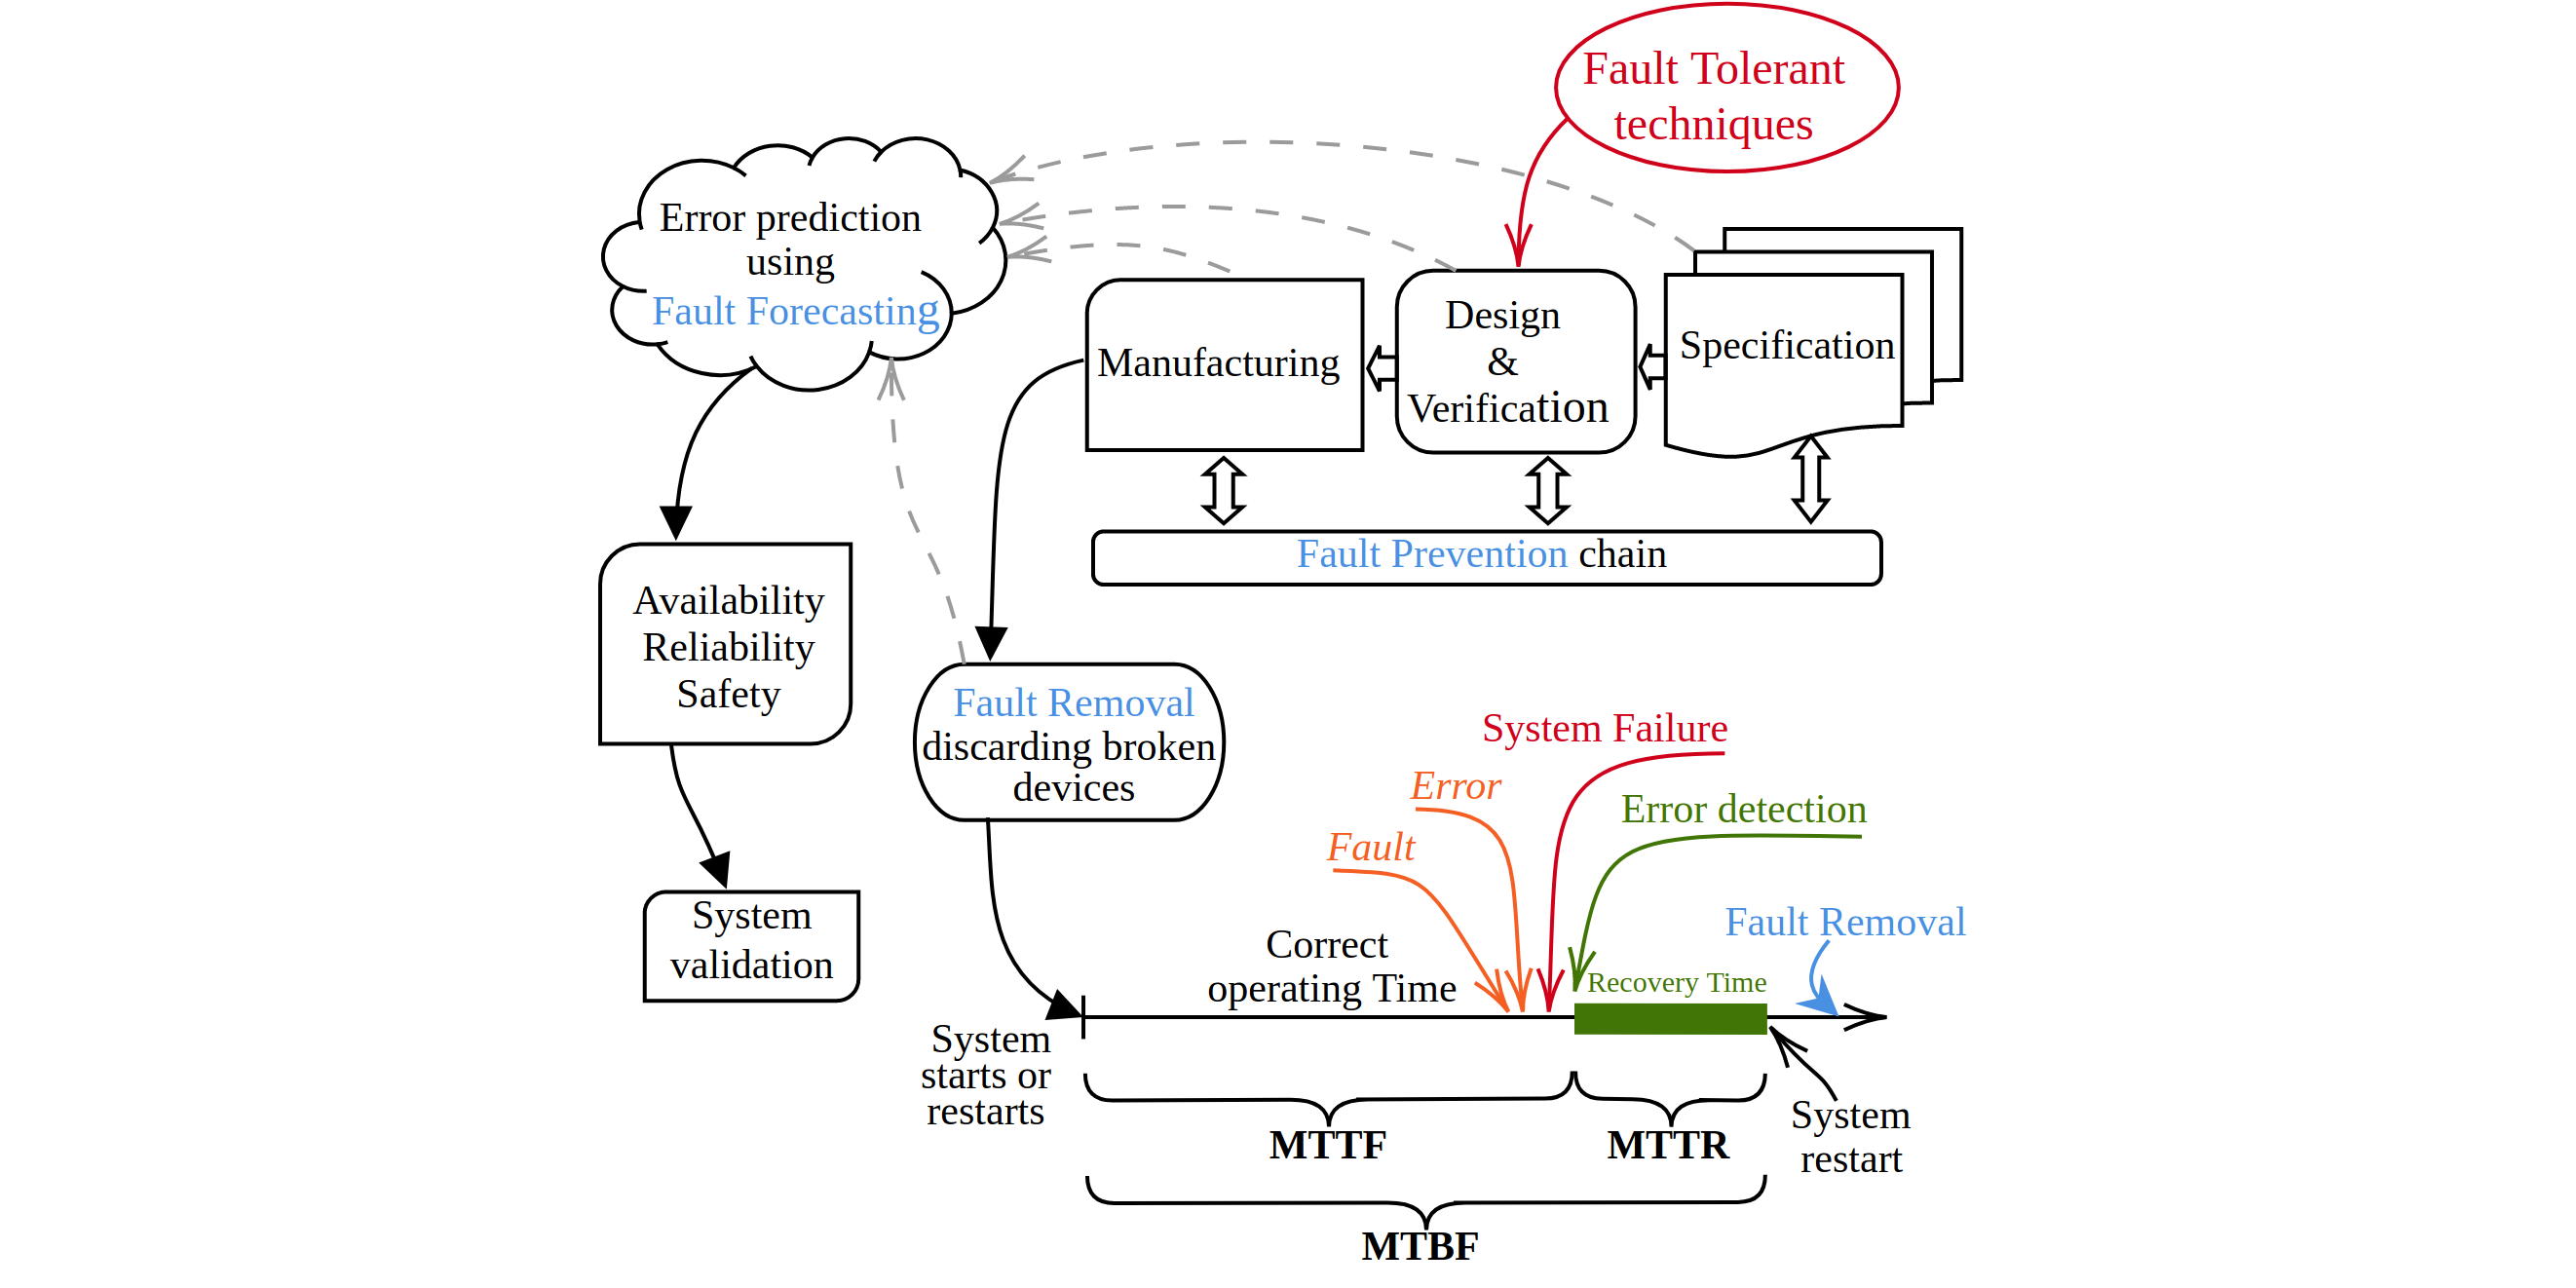
\includegraphics[scale=0.26,center]{./images/Dependability1.png}
				\caption{Design and life of a Dependable System}
				\label{fig:dependability1}
			\end{figure} 
			The block diagram in Figure \ref{fig:dependability1} start with the specification of the system, then the designer use Fault tolerant techniques to design and verify the system, finally the product is manufactured, in these tree steps is applied Fault Prevention in order to reduce unwanted errors. After manufacture, the manufacturer apply a selection in order to discard broken devices and finally the systems is sold and it begins to be used. Meanwhile we gather data from all production chain in order to use Fault Forecasting to predict MTTF,MTTR and MTBF. Then using predicted data are evaluated required Dependability Attributes and finally system is validated and can be sold.
			
			When the system begins to be used there are some periods of correct operations (estimated as MTTF), then at a certain instant a fault occur, this fault can propagate in an Error and this can became a System Failure. If the Failure is detected the system begins the Recovery Time ( estimated as the MTTR ) in which the failure is fixed. In the diagram we select a time interval in which fault is propagated but in a Dependable system this should happen rarely. It is also indicated the removal of defected parts using Fault Removal, this techniques can be also applied during Recovery time.  
			     
			In the next section we contextualize this thesis work analyzing the parts of a critical electronic system.
		} % end Dependability Model
	
	
		\subsection{Electronic system parts}{
			% Article & books
			% Chapter 5 of : ECSS Space product assurance
			% 
			This section describe how this Thesis is positioned in a complete dependable electronic system.
			In figure \ref{fig:ElectronicSystemParts} we give an example of electronic system, it receives information from \textit{sensors} and it controls some \textit{actuators} according to their specification. The circuit is powered by a battery or by power network and this energy should be converted inside the board to be used. For this reason there is a part of the PCB dedicated to \textit{voltage conversion}, this block is composed by analogue and digital components that together create the Power Conversion and Distribution system.
			
			\begin{figure}[H]
				\centering
				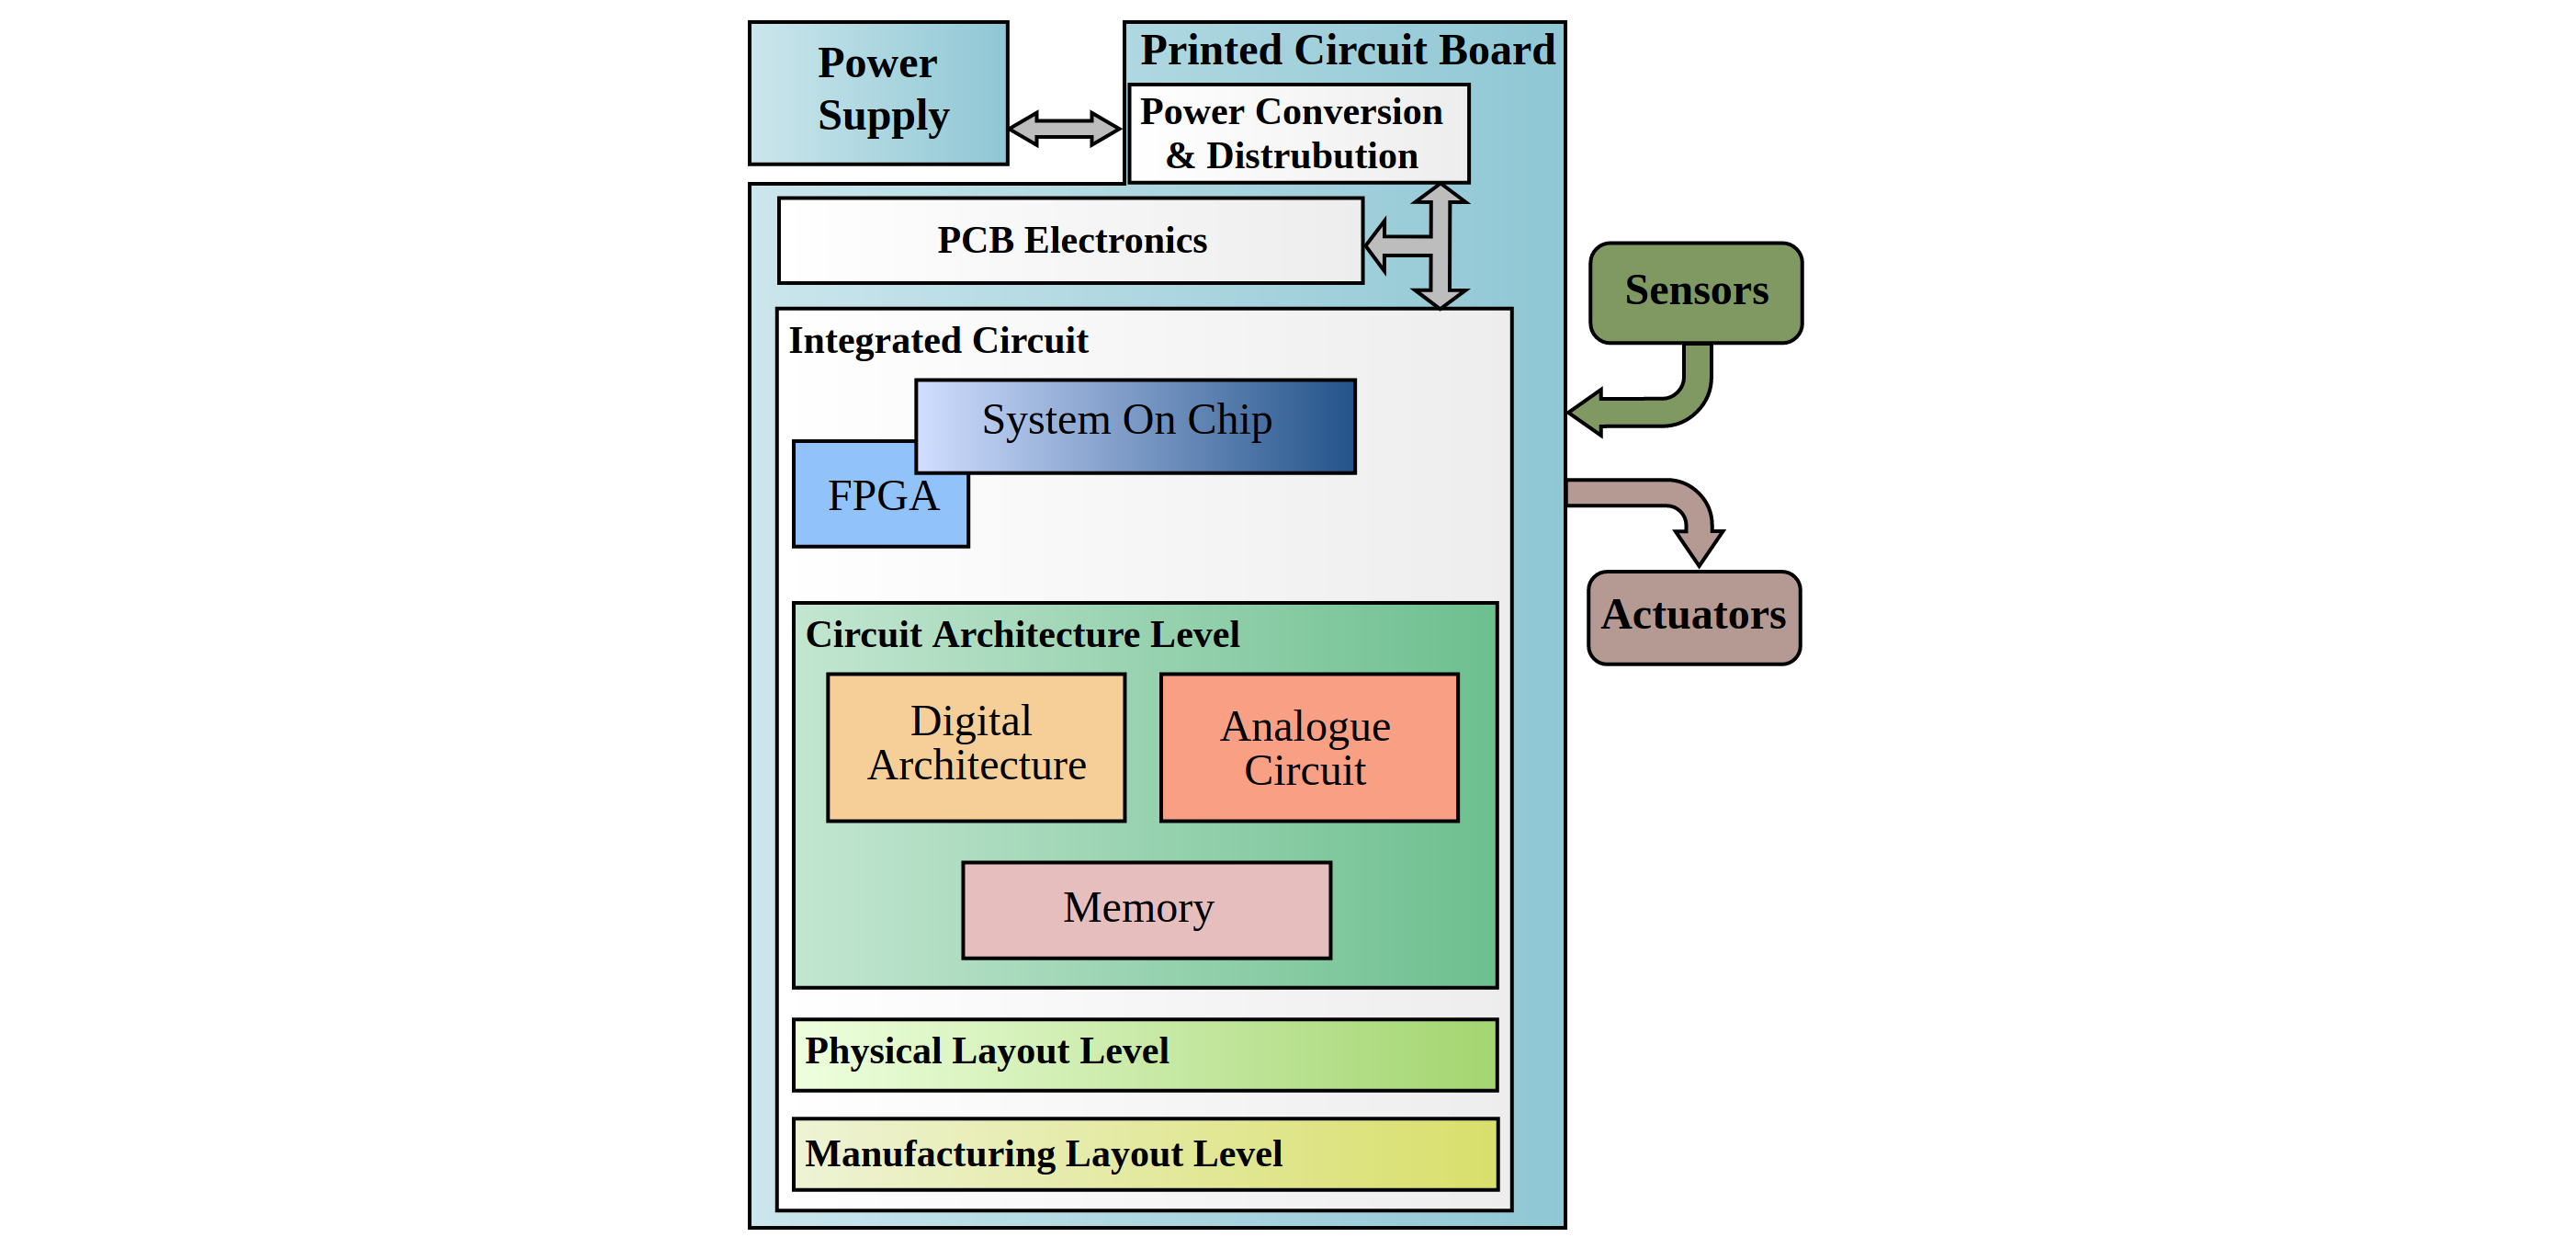
\includegraphics[scale=0.26,center]{./images/ElectronicSystemParts.png}
				\caption{Example of Electronic System}
				\label{fig:ElectronicSystemParts}
			\end{figure} 
			
			The elaboration part instead is composed by integrated circuits that analyze the data received from analog and digital sensors and they use this data to decide how to control the actuators. This elaboration is done by a microcontroller or an FPGA and the design of these ICs have four main design level \cite{ECSS2016} as you can see in Figure \ref{fig:ElectronicSystemParts}:
			\begin{itemize}
				\item \textbf{Manufacturing Process Level } (lev. 4) : This is the level of manufacturing processes, in this step are defined all technique to create the die from a silicon wafer. In the case of hardened chip the manufacturer apply fault tolerant and fault prevention techniques in order to improve system dependability. 
				\item \textbf{Physical Layout Level} (lev. 3) : It is the set of techniques used to place transistors properly. In the case of robust systems the layout is improved in order to decrease the sensitivity of the circuit to radiation.
				\item \textbf{Circuit Architecture Level } (lev. 2) : At this level circuits design is carried out at the RTL level; the circuits may be digital, analogue or a mixed signal. Generally to make this level robust are used fault tolerance redundancy and error correction techniques.   
				\item \textbf{Electronic System Level } (lev. 1) : In this case we can still work at the RTL level using components previously created at the architectural level, or at the unit level (e.g. cluser computers). In the case of robust systems is used processor redundancy (e.g. lockstep technique) or redundancy of computers.
			\end{itemize}  
		
		
			As we have seen, an electronic system is made up of many parts which must all be dependable in order to have a dependable system. \textit{This Master Thesis will deal with the second design level, which is the architectural one}. In order to be able to use the proposed rtl project correctly, it is necessary to use hardening techniques in all the lower and higher levels. In fact what is important for the final application is the depandability of the system, so it would be almost useless to use a hardened processor in a device where the power supply part is not dependable.
		
		} % end Electronic system parts
		\subsection{IEC61508 Standard}{
			% Article & books
			% articolo: iec61508_overview
			% documenti dello standard
			
		} % end IEC61508 Standard
	}% end Safety critical application system
	\section{Dependability of Integrated Circuits}{
		% Article & books
		% Case study in chapter 8 of : (book) Fault tolerant Systems
		
		\subsection{Physical origins and mechanisms of faults}{
			% Article & books
			% intro of: (book) Fault Tolerant Computer Architecture
			% Chapter 2 of : (book) Fault tolerant Systems
			% Defect Tolerance in VLSI Circuits chapter 10 of : (book) Fault tolerant Systems
			% Cyber-Physical System Chapter 7 of : (book) Fault tolerant Systems
			% Introduction (for cosmic rays) : Fault‐Tolerance Techniques for Spacecraft Control Computers
			% Radiation Effects in a Post-Moore World
			Faults in integrated circuits are due to both bit flip or electrical problems such as broken interconnects. The origins of these problems are due both to the aging of integrated transistors and their susceptibility to charge injection by external particles, such as cosmic rays.
			
			
			These two phenomena are influenced by the field of use of the IC and by the working conditions. For example, aging is accelerated by high temperatures and high workloads, which wear out the interconnections. On the other hand the influence of external particles increases in space applications due to the increased cosmic ray flux, as well as in nuclear power plants or where some radioactive materials are present.
			
			
			\textit{The understanding of these phenomena is essential to improve fault tolerance techniques applied to integrated circuits also at RTL level}, therefore the causes and mechanisms of faults are now investigated by dividing them into \textit{internal factors} (due to degradation) and \textit{external factors} (due to particle flux or EMI).
			
			\paragraph{Internal Factors of Faults}{
				As already mentioned, the internal factors of faults are due to electrical problems, which can be caused either by the breakage of the interconnections or by problems related to the gate oxide of the transistors.
				
				As far as interconnections are concerned, there are two origins of failure:
				\begin{itemize}
					\item \textbf{Electromigration} (EM) : EM is a phenomenon known since 1966 \cite{EM1989}, whereby the electrons generating the electric current in the interconnections impart a momentum to the metal atoms. This momentum transfer can create void in the very small interconnections of ICs. The phenomenon is directly proportional to the square of the charge density ($j_e;\;\; [A/cm^2]$) and depends exponentially on the \textit{activation energy} of the material ($E_a;\;\;[eV]$) and on the temperature ($T \;\;\;[K]$). In fact, the Median Time To Failure can be calculated according to the Black's formula \cite{Mukherjee2008}:	
					\begin{equation}
						MeTTF_{system} \;=\; \frac{A_0}{j_e^2}\,e^{\frac{E_a}{kT}} 
					\end{equation}
					Where $A_0$ is a technology dependent constant and k is the Boltzmann constant. 
					
					The opposite effect to EM is due to mechanical stress which tends to compensate for the displacement of metal atoms, this principle is the basis of the Blech effect for which below a certain length (called the Blech length) EM has no effect because the two forces are balanced. Normally the length of the interconnections is greater than the Blech length and for this reason EM is reduced by various techniques. For example, the use of metal alloys (Al+Cu, Al+Pd) or by creating \textit{Bamboo Structures} that reduce the number of metal grains. In fact, the creation of a void in a connection starts at the interface between two or more grains of metal, where the mobility of the atoms is greater and this initial phenomenon leads to an avalanche effect which creates the final voids.
					
					Electromigration create both permanent or intermittent faults and leads the chip in the wear-out phase, it is related to current density that normally depends on workload so fault tolerant strategy that reduce the EM lead with resource multiplexing and oversizing.
					
					\item \textbf{Migration Stress} (MS) : 
					
			\end{itemize}
			}
			\paragraph{External Factors of Faults}{
				
			} 
			
		}% end Origins of faults
		\subsection{Fault classification}{
			% Article & books
			% chapter 4 of: (ECSS) Techniques for radiation effects mitigation in ASICs and FPGAs handbook
			% 1.1 of : (Book) Fault tolerant Systems
			% Introduction (for TID and SEE) : Fault‐Tolerance Techniques for Spacecraft Control Computers
		}% end Fault classification
		\subsection{Masking}{
			% Article & books
			% Chapter on masking: (book) Fault Tolerant Computer Architecture
			
			
		}% end Masking
		\subsection{General Hardening strategy for IC}{
			% Article & books
			% Chapter 2,3,4,5 of : (book) Fault tolerant Systems
			% Chapter 2: Fault‐Tolerance Techniques for Spacecraft Control Computers
		}% end General Hardening strategy for IC
		
	}
	\section{Hardening techniques for digital circuit architectures}{
		% Article & books
		%	
		\subsection{Clock Protection}{
			% Article & books
			%	
			
		}
		\subsection{Logic and Arithmetic circuit protection}{
			% Article & books
			%	
			
		}
		\subsection{Memories protection}{
			% Article & books
			% Information redundancy Chapter 3 of : (book) Fault tolerant Systems
			
		}
		\subsection{Combinational and Sequential circuit protection}{
			% Article & books
			% Chapter 2 and 3 of : (book) Fault tolerant Systems
			
		}
	
	}
	\section{Validation techniques for digital circuit architectures}{
		% Article & books
		%	
		
		\subsection{Real life testing}{
			% Article & books
			%	
			
		}
		\subsection{Ground Accelerated Radiation testing}{
			% Article & books
			%	7
			
		}
		\subsection{Analytical approach}{
			% Article & books
			% Simulation techniques chapter 9 : (book) Fault tolerant Systems
			
		}
		\subsection{Fault Injection (FI)}{
			% Article & books
			% Simulation techniques chapter 9 : (book) Fault tolerant Systems
			% Fault‐Injection Techniques chapter 7: Fault‐Tolerance Techniques for Spacecraft Control Computers
			
		}
	}
}